\documentclass{article}
\usepackage[utf8]{inputenc}
\usepackage[spanish]{babel}
\usepackage{listings}
\usepackage{graphicx}
\graphicspath{ {images/} }
\usepackage{cite}

\begin{document}

\begin{titlepage}
    \begin{center}
        \vspace*{1cm}
            
        \Huge
        \textbf{Desafio 1}
            
        \vspace{0.5cm}
        \LARGE
        Informa2 S.A.S
            
        \vspace{1.5cm}
            
        \textbf{Victor Manuel Jimenez Garcia\\
                Jose Miguel Jaramillo Sanchez\\
                Sebastian Garcia Morales}

        \vfill
            
        \vspace{0.8cm}
            
        \Large
        Despartamento de Ingeniería Electrónica y Telecomunicaciones\\
        Universidad de Antioquia\\
        Medellín\\
        Febrero 17 de 2022
            
    \end{center}
\end{titlepage}

\tableofcontents

\newpage
\section{Objetivos}\label{objetivos}
\begin{itemize}
    \item Aplicar los conocimientos adquiridos a lo largo del curso, demostrando apropiación de los fundamentos básicos del lenguaje de programacion C++.
    \item Desarrollar habilidades de investigación y redacción que permitan la adquisicion de nuevos conocimientos con el fin de solucionar problemas de la vida real.
    \item Demostrar la importancia y utilidad de la programación por hardware, así como el uso de módulos físicos para optimizar el uso de software en un diseño
    \item Diseñar un aplicativo en la plataforma de Arduino integrando programación de C++ para solucionar un desafio  propuesto.
\end{itemize}
\section{Introduccion}\label{intro}
\section{Marco Teorico}\label{marco}

\subsection{Conocimientos previos}

A la hora de enfrentarse a un desafío lo más recomendable es dividirlos en varias etapas para trabajarlo más fácilmente, una primera etapa sería realizar una investigación de conceptos y componentes propuestos en el desafío. En este caso es necesario investigar el concepto de transferir información de forma serial y paralela cómo también identificar características, funcionalidades arquitectura, conexiones, alcances y limitaciones del circuito integrado 75HC595, por otro lado, ¿qué es un Arduino? y ¿cómo unirlo al circuito integrado mencionado anteriormente para lograr solucionar el desafío completo?

El sistema de encriptacion intercambia informacion por medio de la comunicacion serial, que es el proceso de enviar datos de caracter binario un bit a la vez.

Para desencriptar, es necesario paralelizar dicha secuencia de bits que luego seran las entradas de un circuito de logica combinacional encargado de comparar los datos de acuerdo a los parametros de desencriptacion.

Paralelizar no es mas que llevar la secuencia de bits que se desplazan como una sola fila, y transformarla en una columna. De esta forma si se tiene una secuencia serial de n bits, al paralelizar, el resultado es una columna de bits de n filas.

Esta accion de paralelizar la llevará acabo el circuito integrado 74HC595 tambien conocido como Registro de desplazamiento. Un chip con 3 entradas y 8 salidas digitales que permitirá, gracias a su diseño, que toda la información que se envíe de manera serial no se muestre en cada una de las salidas, es decir, que la información que se requiera enviar para una determinada salida en particular,se mostrará únicamente ahí y no en las demás, ya que el pulso que se envíe desde la entrada deberá pasar por cada una de las salidas del circuito hasta llegar al destino, pero al contar con un Buffer en cada salida, se consigue controlar las transiciones de modo que solo se observe cuando llegue a la salida destino deseada.


\begin{figure}[!ht]
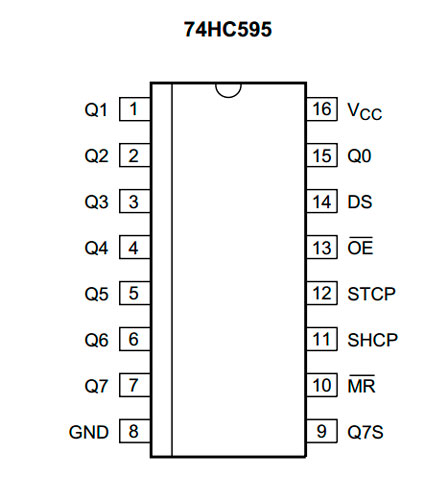
\includegraphics[width=5cm]{74HC595.jpg}
\centering
\caption{Pines IC 74HC595}
\end{figure}

\noindent\textbf{Salidas:}\\ 
\indent Q0-Q7 (pines 1-7 y 15 )\\
\textbf{Entradas:}\\
\indent DS: entrada de datos (pin 14)\\
\indent STCP: entrada de la señal de reloj (pin 12)\\
\indent SHCP: entrada del pulso para liberar los datos (pin 11)


\section{Analisis del problema} \label{analisis}



\section{Conclusiones} \label{conclusiones}


\bibliographystyle{IEEEtran}
\bibliography{references}

\end{document}
